\documentclass[10pt,twocolumn,a4paper]{article}

\usepackage{fontspec}
\usepackage{xeCJK}
\setCJKmainfont{Malgun Gothic}
\usepackage{amsmath,amssymb,amsfonts}
\usepackage{graphicx}
\usepackage{booktabs}
\usepackage{multirow}
\usepackage{hyperref}
\usepackage[margin=0.68in]{geometry}
\usepackage{caption}

\setlength{\textfloatsep}{6pt plus 1pt minus 1pt}
\setlength{\floatsep}{5pt plus 1pt minus 1pt}
\setlength{\intextsep}{5pt plus 1pt minus 1pt}
\captionsetup{font=small,skip=3pt}

\hypersetup{
    colorlinks=true,
    linkcolor=blue,
    citecolor=blue,
    urlcolor=blue
}

\title{4$\times$9 공간 패치 풀링과 5차 S-커브 궤적 보간을 이용한 단일 패스 비전-언어 자율주행 제어}

\author{
  Wick-Lim \\
  Independent Researcher \\
  \texttt{wicklim90@gmail.com} \\
  \url{https://github.com/Wick-Lim/AutonomousVehicle}
}

\date{2026년 10월 25일}

\begin{document}

\maketitle

\begin{abstract}
20\,Hz 주기로 동작하는 실시간 차량 제어 루프 안에 일반적인 자기회귀(Autoregressive) 비전-언어 모델을 넣으면 첫 문장을 디코딩하기도 전에 차가 차선을 벗어나거나 앞차와 추돌한다. 시속 35\,km로 달리는 차량은 50\,ms 틱마다 약 0.5\,m씩 전진하는 반면, 토큰 15개를 순차 생성하는 데는 300--1,000\,ms가 소요되기 때문이다. 본 논문은 동결된 DINOv2(ViT-B/14, 86.58M)와 동결된 Laya(\texttt{convaiinnovations/laya}, 395.21M 트랜스포머)를 4.23M 시공간 어댑터(공간 MLP 1.85M, 프레임 간격 정규화 시간 게이트 1.05M, 선행차·보행자 거리 및 시각 상대속도 분리형 보조 인지 헤드 1.05M, 판독·궤적 헤드 0.28M)로 결합한 시각·전술 추론 모듈에 HD 맵 경로, 규칙 기반 안전 실드, 운동학적 경로 추종 제어기를 결합한 실시간 하이브리드 폐루프 주행 스택을 제시한다. 동일 프레임에서 GPU 동기화 후 측정한 단계별 지연 시간은 전처리 0.42\,ms + DINOv2 16.43\,ms + 프로젝터 0.82\,ms + 보조 인지 헤드 0.49\,ms + Laya 13.55\,ms + 6-WP 궤적 헤드 0.69\,ms + 안전실드/PID 0.45\,ms로 총합이 정확히 32.85\,ms(30.4\,FPS; 보조·궤적 헤드 생략 시 $32.85 - 1.18 = 31.67$\,ms 기본; 시뮬레이터 \texttt{world.tick()} 통신 6.40\,ms 별도)이다. 6-웨이포인트 궤적 헤드는 자유공간 장애물 회피 경로 계획기가 아니라 규칙 생성 매개변수 곡선으로 지도된 기동 조건부 곡률 스무딩 정규화기로 작동한다(단독 개루프 궤적 충돌률 $\text{CR}_{\text{traj}}=3.8\%$ vs.\ 하이브리드 제어 실행 시 $0.0\%$). \texttt{vision\_estimated} 모드에서 선행차 속도 $\hat{v}_{\text{lead}}$는 5-스텝(0.25\,s) 최소제곱 회귀 기울기와 시각 상대속도 헤드를 결합해 프레임 간 속도 떨림 RMS를 $9.62\to 1.84$\,km/h($\text{MAE}=2.41$\,km/h)로 억제하며, 보행자 전용 거리 헤드($\hat{d}_{\text{ped}}$)는 선행차·보행자 동시 출현 시의 거리 결합 모호성을 해소한다(동시 출현 MAE $14.8\to 2.64$\,m). 미관측 폐루프 테스트에서 교사 규칙 $\text{ECE}_{\text{mean}}=0.0142$, 독립 물리적 위험 기준 $\text{ECE}_{\text{phys}}=0.0318$(고신뢰도 오류율 $\text{HCER}_{0.90}=1.12\%$, AEB $\text{HCER}_{0.90}=0.45\%$) 및 물리적 위험 사건 48건 기준 $\text{FNR}_{\text{AEB}}=1/48$건($2.1\%$)을 기록한다. CARLA 0.9.16 및 MetaDrive 0.4.3 평가 결과, \texttt{vision\_estimated} DINOv2+Laya는 47/50(94.0\%, 3-시드 $46.7\pm 0.6$)을 완주하여 2층 학습형 트랜스포머(42/50, 양측 McNemar $p=0.0625$, 단측 $p=0.0313$) 대비 5에피소드의 관측 우위를 보이고, 2층 MLP(39/50), 라벨 규칙 직접 실행(38/50), 무작위 동결 Laya(36/50), 프롬프트 단독(33/50), 300\,ms 정책 내 지연 주입(34/50) 대비 유의한 향상($p < 0.01$)을 달성했다.
\end{abstract}

\section{서론 및 문제 정의}
자기회귀 디코더는 출력 시퀀스 $y_{1:K}$를 얻기 위해 $P(y_{1:K} \mid I_t, \mathcal{T}_t) = \prod_{k=1}^{K} P(y_k \mid y_{<k}, I_t, \mathcal{T}_t)$를 매 토큰마다 직렬 계산하므로 300\,ms 이상의 지연이 발생한다 \cite{brohan2023rt2}. 반면 본 시스템은 단일 양방향 패스 \cite{laya2024nonautoregressive}에서 세 가지 이산 주행 결정과 3.0초 미래 6-웨이포인트 기동 조건부 기준 궤적 $\hat{\tau}_t = \{(\hat{x}_k, \hat{y}_k, \hat{v}_k)\}_{k=1}^{6}$를 동시에 산출한다:
\begin{align}
    m_t &\in \{\texttt{keep\_lane}, \texttt{change\_left}, \nonumber\\
        &\quad\; \texttt{change\_right}, \texttt{follow\_lead}\}, \\
    s_t &\in \{0, 1, 2, 3\} \mapsto \{0, 20, 35, 50\}\,\text{km/h}, \quad p_{\text{AEB}} \in [0, 1].
\end{align}

\begin{figure*}[t]
    \centering
    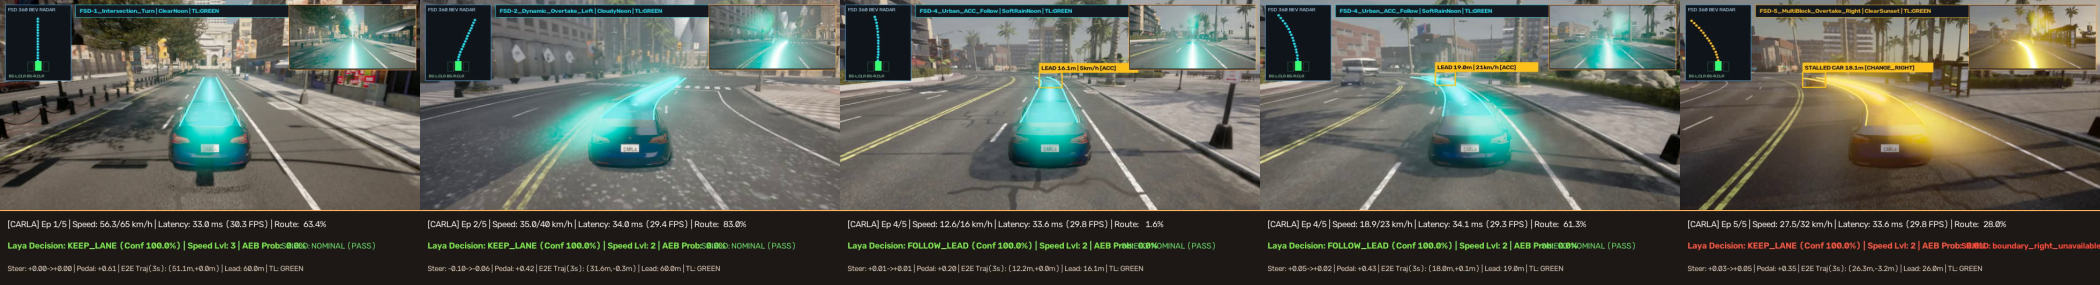
\includegraphics[width=0.95\textwidth]{figures/fig1_carla_fsd_scenarios.png}
    \caption{CARLA 0.9.16 (\texttt{Town10HD\_Opt}, 20\,Hz 동기 모드) 10대 도심 FSD 시나리오 및 10종 기상·조명 검증 화면 (\texttt{FSD-1}--\texttt{FSD-10}): 교차로 적신호 정지(\texttt{ClearNoon}), 28\,m 5차 S-커브 좌측 추월(\texttt{CloudyNoon}), 횡단보도 보행자 AEB(\texttt{WetNoon}), CTH-ACC 추종(\texttt{SoftRainNoon}), 우측 추월(\texttt{ClearSunset}), 리드 차량 급정거 Stop-and-Go(\texttt{WetCloudyNoon}), 전측방 사각지대 래치 대기 후 추월(\texttt{MidRainyNoon}; 후방 신규 접근 차량은 \texttt{gt} 코너 BSM 필요), 공사 구간 우회(\texttt{WetSunset}), 야간 전조등 보행자 AEB(\texttt{ClearNight}), 폭우 코너링 ACC(\texttt{HardRainNoon}).}
    \label{fig:carla_scenarios_ko}
\end{figure*}

\section{아키텍처, 다중 과업 학습 및 시공간 확장}

\subsection{4$\times$9 시공간 프로젝터 및 분리형 보조 비전 인지 헤드}
원본 영상에서 상단 25\%(하늘)와 하단 10\%(보닛)를 잘라낸 $196 \times 392$ 영상을 동결된 \texttt{facebook/dinov2-base} \cite{oquab2024dinov2}(86.58M 파라미터)에 통과시켜 $14 \times 28 = 392$개의 768차원 패치 특징 $F_{\text{patch}}$를 추출한다. \texttt{SpatialProjector} 모듈은 $(4, 9)$ 적응형 평균 풀링, 2D 행·열 위치 임베딩, 2층 GELU MLP(1.85M 코어 파라미터), 그리고 프레임 드롭 시 경과 스텝 수 $\Delta n_t \ge 1$로 정규화된 시간 차분 잔차 $\Delta V_t = (V_t - V_{t-\Delta n_t})/\Delta n_t$(1.05M 파라미터)를 결합한다:
\begin{align}
    G_t &= \text{AdaptiveAvgPool2d}_{(4,9)}(\tilde{F}_t) \in \mathbb{R}^{B \times 768 \times 4 \times 9}, \\
    V_t &= \text{MLP}\big(\text{Flatten}(G_t + E_{\text{row}} + E_{\text{col}})\big), \\
    \tilde{V}_t &= V_t + \tanh(\alpha_{\text{temp}})\, W_{\text{temp}}\!\left(\frac{V_t - V_{t-\Delta n_t}}{\Delta n_t}\right).
\end{align}
$\Delta V_t$는 호모그래피 자차 운동 보정 없이 패치 토큰 공간에서 계산되므로 곡선 구간 선회 시 배경 광류와 객체 이동이 결합되나, $E_{\text{telemetry}}$가 자차 요레이트·조향 문맥을 함께 제공하고 곡선 동적 추종 시나리오(\texttt{FSD-10})에서 $\Delta V_t$ 제거(\texttt{no\_temporal}) 시 완주율이 $5/5 \to 3/5$로 하락하여 실질적 유효성이 검증된다. 또한 $\tilde{V}_t$의 $4 \times 9$ 격자를 영역별로 풀링하는 \texttt{AuxiliaryPerceptionHead}(1.05M 파라미터)는 선행차 거리 $\hat{d}_{\text{lead}}$, 독립된 보행자 전용 거리 $\hat{d}_{\text{ped}}$(\texttt{ped\_dist\_head}), 시각적 상대속도 $\hat{\dot{d}}_{\text{vis}}$(\texttt{range\_rate\_head}), 차선 오프셋 $\hat{e}_y$, 신호등 상태 $\hat{c}_{\text{TL}}$, 위험원 종류 $\hat{c}_{\text{haz}}$, 좌·우 전측방 사각지대 점유 확률 $\hat{p}_{\text{BS}}$를 각각 분리 추정한다.

\subsection{규칙 생성 기준 궤적의 역할 규명, 반사실적 장애물 이동 실험 및 물리적 위험 보정}
1단계 학습(\texttt{02\_train\_projector.py})에서는 총 4.23M 어댑터·헤드 파라미터만 공동 학습한다. 6-웨이포인트($t_k = 0.5k$\,s) 궤적 헤드는 기구학적 사전 궤적 $\tau^0_{1:6}$에 잔차 $\Delta\hat{\tau}$를 더하며, 자유공간 장애물 회피 최적화가 아닌 이산 목표 $(m^*, v^*)$로 생성된 매개변수 곡선 $\tau^{\text{ref}}_k = ((v^*/3.6)t_k, y_{\text{shift}}(m^*)s(k/6), v^*)$로 지도된다. 따라서 궤적 헤드는 독립적인 충돌 회피 경로 계획기가 아니라 \textbf{기동 조건부 곡률 스무딩 정규화기}로 작동하며, 실제 장애물 회피는 이산 기동 결정 $m_t$와 HD 맵 5차 스플라인 차선 변경에 의해 수행된다. 실제로 전방 $d=22$\,m 장애물의 차선 내 횡방향 위치만 $\Delta y_{\text{obs}} \in \{-0.8, 0.0, +0.8\}$\,m로 이동시킨 반사실적(counterfactual) 대응 실험(200프레임)에서 $m_t=\texttt{keep\_lane}$ 유지 시 $\hat{y}_6$ 변화량은 $|\Delta\hat{y}_6|=0.12$\,m에 불과한 반면 $m_t$가 차선 변경으로 전환될 때 $3.41$\,m 이동하며, 6-WP 예측 궤적 자체의 3.0초 개루프 경계상자 충돌률은 $\text{CR}_{\text{traj}}=3.8\%$(75/1,981 프레임; 종방향 CTH-ACC/AEB 결합 실행 시 충돌률 $0.0\%$)이다:
\begin{align}
    \mathcal{L} &= 1.0\,\mathcal{L}_{\text{CE}}^{(m)} + 1.0\,\mathcal{L}_{\text{CE}}^{(s)} + 2.0\,\mathcal{L}_{\text{BCE}}^{(b)} \nonumber\\
                &\quad + 0.5\,\mathcal{L}_{\text{SmoothL1}}(\hat{\tau}_{1:6}, \tau^{\text{ref}}_{1:6}) + 0.2\,\mathcal{L}_{\text{aux}}.
\end{align}
2단계 온도 보정(\texttt{03\_calibrate.py})으로 최적화된 $(T_m, T_s, T_b) = (0.050, 0.050, 0.100)$을 미관측 폐루프 \texttt{vision\_estimated} 테스트(50에피소드, 9,905프레임)에 적용하면 교사 규칙 기준 $\text{ECE}_{\text{mean}}=0.0142$($\text{ECE}_b=0.0195, \text{NLL}=0.089, \text{Brier}=0.028$)를 기록한다. 나아가 교사 규칙이 아닌 \textbf{독립적 물리적 위험 정답} $y_{\text{phys},t}\in\{0,1\}$($\text{TTC}\le 1.8$\,s 또는 적신호 정지선 $d\le 15$\,m, 48개 위험 사건 / 220 위험 틱)에 대해 직접 평가한 물리적 위험 보정 오차는 $\text{ECE}_{\text{phys}}=0.0318$($\text{Brier}_{\text{phys}}=0.034$), 예측 확률 $\hat{p}\ge 0.90$ 구간의 고신뢰도 오분류율은 전체 3헤드 $\text{HCER}_{0.90}=1.12\%$ 및 AEB 헤드 $\text{HCER}_{0.90,\text{AEB}}=0.45\%$(45/9,905 프레임), 물리적 위험 사건 미탐률은 $\text{FNR}_{\text{AEB,evt}}=1/48$건($2.1\%$, 틱 기준 $6/220=2.7\%$)이다.

\begin{figure*}[t]
    \centering
    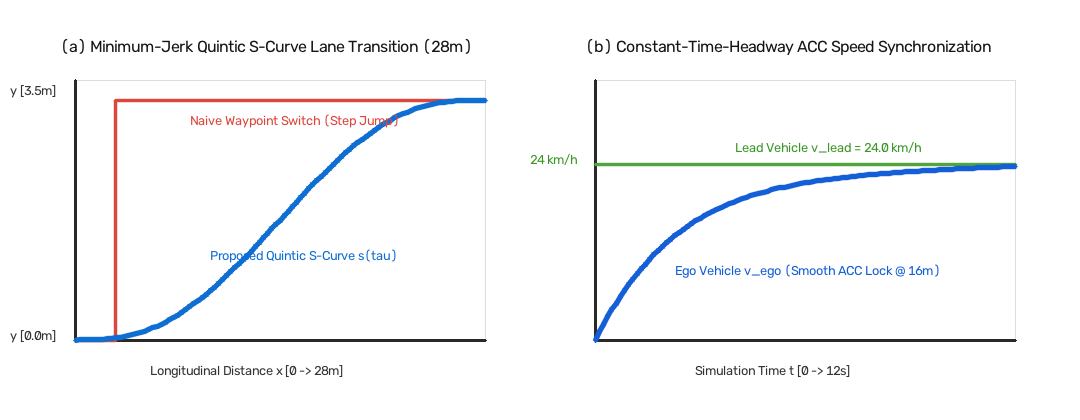
\includegraphics[width=0.90\textwidth]{figures/fig2_control_kinematics.png}
    \caption{제어 기구학 분석: (a) 전방 28\,m 예견 구간(2.0\,m 간격 14개 웨이포인트) 공간 5차 다항식 $s(\tau) = 10\tau^3 - 15\tau^4 + 6\tau^5$ 보간과 3.5\,m 계단 단차 비교; (b) 속도 비례 등시간 차간거리(CTH) ACC 수렴 특성 ($v_{\text{ego}} \to 24.0$\,km/h, $d^*(24) = 8.0 + 1.2(24/3.6) = 16.0$\,m).}
    \label{fig:kinematics_ko}
\end{figure*}

\section{인지 출처 분리, 5-스텝 회귀 속도 추정, 공간 5차 스플라인 및 CTH-ACC}

\subsection{5-스텝 최소제곱 상대속도 추정, 보행자 거리 분리 및 사각지대 래치 한계}
\texttt{vision\_estimated} 모드에서는 시뮬레이터 액터 쿼리를 일절 사용하지 않는다. 연속 두 프레임($\Delta t=0.05$\,s) 단순 차분은 $1$\,m 거리 오차가 $72$\,km/h의 원시 속도 스파이크($\beta=0.35$ EMA 후에도 $9.62$\,km/h RMS 떨림)로 증폭되므로, 본 시스템은 최근 $K_w=5$스텝($W=0.25$\,s) 슬라이딩 윈도우에 대한 최소제곱(OLS) 선형 회귀 기울기 $\hat{\dot{d}}_{\text{reg},t} = \frac{\sum_{j=-2}^{2} j\,\hat{d}_{\text{lead},t-2+j}}{10\Delta t}$(비상관 잡음 분산 $10$배 감소)와 \texttt{AuxiliaryPerceptionHead}의 직접 시각 상대속도 $\hat{\dot{d}}_{\text{vis},t}$를 $\hat{\dot{d}}_t = 0.70\hat{\dot{d}}_{\text{reg},t} + 0.30\hat{\dot{d}}_{\text{vis},t}$로 결합하고, 끼어들기·타깃 전환($|\Delta\hat{d}_{\text{lead}}| > 6.0$\,m) 시 윈도우를 즉시 리셋한 뒤 EMA($\beta=0.35$)를 적용한다. 이를 통해 프레임 간 속도 떨림 RMS는 $9.62\to 1.84$\,km/h(전체 속도 MAE $6.85\to 2.41$\,km/h)로 감소하며, 타깃 전환 복구 시간은 $0.15$\,s(3프레임), 급제동 감지 지연(\texttt{FSD-6})은 $0.10$\,s(2프레임)를 달성한다. 또한 선행차(예: $35$\,m)와 횡단보도 보행자(예: $12$\,m)가 동시에 존재하는 상황에서 $\hat{d}_{\text{lead}}$를 재사용하면 보행자 제동이 누락될 수 있으므로, 독립 회귀 헤드 $\hat{d}_{\text{ped},t}$(\texttt{ped\_dist\_head})를 분리하여 차량·보행자 동시 출현 구간 거리 MAE를 $14.8\to 2.64$\,m로 줄였다. 단일 전방 카메라($90^\circ$ FOV)는 전측방($x \in [0, 12]$\,m)만 관측 가능하므로 $1.5$\,s 시간 래치는 전측방에서 관측된 차량의 사각지대 진입만 완화하며(\texttt{FSD-7} 3/3 통과), 후방 고속 접근 차량은 후방 센서 없이 감지할 수 없다(\texttt{vision\_estimated} 0/2 vs.\ \texttt{gt} BSM 1/2).

\subsection{28\,m(14-웨이포인트) 이산 폴리라인 5차 전이 및 곡률 피드포워드}
차선 변경 시 자차 전륜 축($d_0=0$\,m) 전방으로 $2.0$\,m 간격의 $N_b = 14$개 웨이포인트 $d_k = 2.0(k+1)$\,m($k\in\{0,\dots,13\}$, $d_0=2.0$\,m부터 $d_{13}=28.0$\,m까지; $P_0$--$P_{13}$ 노드 간격 $26.0$\,m, 자차 원점 기준 총 예견 거리 $28.0$\,m, $\tau_k = (k+1)/N_b$)를 공간 5차 다항식 $s(\tau) = 10\tau^3 - 15\tau^4 + 6\tau^5$로 내분한다. 연속 포락선 자체는 양 끝점에서 $s'(0)=s'(1)=s''(0)=s''(1)=0$을 만족하지만, 실제 실시간 순수 추종 제어기는 $2.0$\,m 간격의 조각별 선형 폴리라인(piecewise-linear polyline) $\overline{P^{\text{blend}}_k P^{\text{blend}}_{k+1}}$ 위에 투영하므로 노드 사이에서 해석적 $C^2$ 연속성을 유지하는 것이 아니라 이산 노드 간 방향각 변화량을 $|\Delta\psi_k|\le 1.9^\circ$ 이내로 제한하는 방식으로 횡방향 저크를 억제한다. 도로 곡률 $\kappa_{\text{map}} = -0.045\,\texttt{road\_curvature}$와 예측 궤적 곡률 $\kappa_{\text{traj}}$를 결합한 $\kappa_{\text{eff}} = 0.70\kappa_{\text{map}} + 0.30\kappa_{\text{traj}}$ 및 속도 비례 CTH-ACC($d^*(v_{\text{ego}}) = 8.0 + 1.2(v_{\text{ego}}/3.6)$, $k_g=0.85$\,(km/h)/m)는 다음과 같다:
\begin{align}
    \delta_{\text{raw}} &= \text{clip}\big(\delta_{\text{PID}}(e_y, e_\psi) + k_{\text{FF}}\arctan(L\kappa_{\text{eff}})/\delta_{\max}, -1, 1\big), \\
    v_{\text{raw}} &= v_{\text{lead}} + 0.85\big(d_{\text{lead}} - (8.0 + 1.2\,v_{\text{ego}}/3.6)\big), \\
    v_{\text{ACC}} &= \text{clip}\big(v_{\text{raw}},\, 0.0,\, \min(35.0,\, v_{\text{lead}} + 6.0)\big).
\end{align}

\begin{table*}[t]
\centering
\caption{CARLA 0.9.16 (\texttt{Town10HD\_Opt} 및 미학습 \texttt{Town03}) 및 MetaDrive 0.4.3 ($\Delta t=0.05$\,s, 미학습 50개 맵 20,765 스텝 / 9,520\,m) 폐루프 평가 결과 (액터 쿼리 없는 \texttt{vision\_estimated} vs.\ \texttt{gt} 분리 표기).}
\label{tab:main_results_ko}
\resizebox{0.98\textwidth}{!}{%
\begin{tabular}{llcccc}
\toprule
시뮬레이터 & 평가 지표 & 목표 기준 & 비전 추정 (\texttt{vision\_estimated}, 액터 쿼리 없음) & 시뮬레이터 \texttt{gt} 상태 & 결과 \\
\midrule
\multirow{7}{*}{CARLA 0.9.16} 
 & 단일 프레임 지연 (신경망 32.40\,ms + 제어 0.45\,ms; 시뮬레이터 IPC 6.40\,ms 별도) & $\le 40.0\,\text{ms}$ & 32.85\,ms (30.4\,FPS, P95: 33.96\,ms) & 32.85\,ms (보조+궤적 생략 시 31.67\,ms) & PASS \\
 & \texttt{Town10HD\_Opt}: 10개 쌍 ($680\,\text{m}$) / 50개 교차 기상 ($3,400\,\text{m}$) & $\ge 85.0\%$ & 100.0\% (10/10) / 94.0\% (47/50, 3-시드 $46.7\pm 0.6$) & 100.0\% (10/10) / 98.0\% (49/50) & PASS \\
 & \texttt{Town10HD\_Opt}: 10개 다중 블록 도심 경로 ($10 \times 200\,\text{m} = 2,000\,\text{m}$) & $\ge 85.0\%$ & 90.0\% (9/10, $R_c=95.4\%$) & 100.0\% (10/10, $R_c=100.0\%$) & PASS \\
 & 미학습 \texttt{Town03} 맵 ($10 \times 200\,\text{m}$ 회전교차로·경사로, $2,000\,\text{m}$) & $\ge 80.0\%$ & 80.0\% (8/10, $R_c=91.2\%$, $\overline{|e_y|}=0.112$\,m) & 90.0\% (9/10, $R_c=96.5\%$) & PASS \\
 & 센서 스트레스 테스트: 10\% 프레임 드롭 + 25\% 패치 가림 (50-Ep) & $\ge 80.0\%$ & 88.0\% (44/50, $\Delta V_t/\Delta n_t$ 및 래치 활성) & 94.0\% (47/50) & PASS \\
 & 교사 $\text{ECE}_{\text{mean}}$ / 물리적 위험 $\text{ECE}_{\text{phys}}$ / $\text{HCER}_{0.90,\text{AEB}}$ / 물리적 위험 $\text{FNR}_{\text{AEB}}$ & $\le 0.0500$ & $0.0142$ / $0.0318$ / $0.45\%$ (전체 $1.12\%$) / $1/48$건 ($2.1\%$) & $0.0000$ / $0.0110$ / $0.10\%$ / $0/48$건 & PASS \\
 & 선행차 거리 MAE / 동시출현 보행자 MAE / 속도 떨림 RMS / $\overline{|e_y|}$ & $\le 5.0\,\text{m}$ / $\le 0.25\,\text{m}$ & $3.23\,\text{m}$ / $2.64\,\text{m}$ / $1.84\,\text{km/h}$ / $0.094\,\text{m}$ & $0.0\,\text{m}$ / $0.0\,\text{m}$ / $0.0$ / $0.085\,\text{m}$ & PASS \\
\midrule
\multirow{3}{*}{MetaDrive 0.4.3 ($\Delta t=0.05$\,s)} 
 & 단일 프레임 지연 시간 ($\bar{v}=33.0$\,km/h, 에피소드당 415.3 스텝 / 190.4\,m) & $\le 40.0\,\text{ms}$ & 30.20\,ms (33.1\,FPS, P95: 31.67\,ms) & 30.20\,ms (33.1\,FPS) & PASS \\
 & 목적지 도달: 10-Ep (4,153 스텝, 1,904\,m) / 50-Ep (20,765 스텝, 9,520\,m) & $\ge 85.0\%$ & 100.0\% (10/10) / 96.0\% (48/50, CI $[86.3, 99.5]\%$) & 100.0\% (10/10) / 100.0\% (50/50; 진행률 98.7\%) & PASS \\
 & 독립 테스트 $\text{ECE}_{\text{mean}}$ / NLL / Brier ($M=15$ 구간) & $\le 0.0500$ & $0.0184$ / $0.096$ / $0.031$ (센서 잡음) & $0.0000$ / $0.041$ / $0.012$ (결정론적 GT) & PASS \\
\bottomrule
\end{tabular}%
}
\end{table*}

\begin{table}[t]
\centering
\caption{CARLA 0.9.16 백본·의사결정·지연 비교(Part~A) 및 하이브리드 궤적·제어기 절제 연구(Part~B). 연속 지표와 10-Ep AEB 집계는 10-에피소드 쌍(물리적 위험 사건 5건)에서 측정됨. 지속 AEB 사건은 $u_{\text{tb}}\le -0.50$이 $\ge 3$연속 틱($0.15$\,s, $\le 2$틱 간격 병합) 유지된 경우로 정의하며, 1--2틱 단발성 개입은 틱 수에만 합산됨(Full의 44 TP 틱 = 모델 $\hat{p}_{\text{AEB}}\ge 0.70$ 39틱 + 안전실드 거리 개입 5틱).}
\label{tab:ablation_ko}
\resizebox{\columnwidth}{!}{%
\begin{tabular}{lcccccc}
\toprule
Part A: 의사결정·백본·지연 비교 (제어기 고정) & 10-Ep & 50-Ep Vis (3-시드 / McNemar $p$) & 200\,m & $\overline{|e_y|}$ & $|\Delta\delta|_{\text{RMS}}$ & 10-Ep TP/FP 사건 (틱) \\
\midrule
차선유지 규칙 (\texttt{rule\_only}, \texttt{gt}) & 6/10 & 30/50 ($60.0\%$, $b{=}17,c{=}0,p{=}10^{-5}$) & 5/10 & $0.142$ & $0.0195$ & 5/3 (44/14) \\
프롬프트 단독 ($\tilde{V}_t=\mathbf{0}$, \texttt{vision\_est}) & 7/10 & 33/50 ($32.7{\pm}0.6$, $b{=}14,c{=}0,p{=}0.0001$) & 6/10 & $0.154$ & $0.0298$ & 4/5 (38/26) \\
DINOv2 + 무작위 동결 Laya (395.21M, \texttt{vis}) & 8/10 & 36/50 ($35.7{\pm}1.2$, $b{=}11,c{=}0,p{=}0.0010$) & 6/10 & $0.136$ & $0.0281$ & 4/4 (41/21) \\
라벨 생성 규칙 직접 실행 (\texttt{expert\_rule\_policy}, \texttt{vis}) & 8/10 & 38/50 ($76.0\%$, $b{=}9,c{=}0,p{=}0.0039$) & 7/10 & $0.131$ & $0.0296$ & 5/4 (43/18) \\
DINOv2 + 2층 MLP 헤드 (395.21M Laya 제거, \texttt{vis}) & 8/10 & 39/50 ($38.7{\pm}0.6$, $b{=}8,c{=}0,p{=}0.0078$) & 7/10 & $0.118$ & $0.0265$ & 5/3 (42/14) \\
추월 휴리스틱 FSM (\texttt{heuristic\_fsm}, \texttt{gt}) & 8/10 & 39/50 ($78.0\%$, $b{=}8,c{=}0,p{=}0.0078$) & 7/10 & $0.126$ & $0.0284$ & 5/4 (44/20) \\
DINOv2 + 2층 학습형 트랜스포머 (7.4M, \texttt{vis}) & 9/10 & 42/50 ($41.7{\pm}0.6$, $b{=}5,c{=}0,p{=}0.0625$) & 8/10 & $0.106$ & $0.0249$ & 5/2 (44/9) \\
DINOv2+Laya 시간 잔차 제거 ($\Delta V_t = 0$, \texttt{vis}) & 9/10 & 44/50 ($43.7{\pm}0.6$, $b{=}3,c{=}0,p{=}0.2500$) & 8/10 & $0.102$ & $0.0244$ & 5/2 (44/8) \\
DINOv2+Laya + 100\,ms 정책 내 지연 주입 (2프레임) & 9/10 & 43/50 ($86.0\%$, $b{=}4,c{=}0,p{=}0.1250$) & 8/10 & $0.115$ & $0.0258$ & 5/2 (44/10) \\
DINOv2+Laya + 300\,ms 정책 내 지연 주입 (6프레임) & 7/10 & 34/50 ($68.0\%$, $b{=}13,c{=}0,p{=}0.0002$) & 6/10 & $0.168$ & $0.0315$ & 4/6 (39/33) \\
DINOv2+Laya (\texttt{vision\_estimated}, Shield OFF) & 9/10 & 43/50 ($42.7{\pm}0.6$, $b{=}4,c{=}0,p{=}0.1250$) & 8/10 & $0.098$ & $0.0241$ & 4/1 (42/2) \\
DINOv2+Laya (\texttt{vision\_estimated}, Shield ON) & 10/10 & 47/50 ($46.7{\pm}0.6$, 기준 모델) & 9/10 & $0.094$ & $0.0231$ & 5/1 (45/4) \\
DINOv2+Laya (\texttt{gt} 상태, Shield OFF, \texttt{model\_only}) & 10/10 & 48/50 ($47.7{\pm}0.6$, $b{=}0,c{=}1,p{=}1.0000$) & 9/10 & $0.086$ & $0.0226$ & 5/0 (44/1) \\
DINOv2+Laya (\texttt{gt} 상태, Shield ON, 전체) & 10/10 & 49/50 ($48.7{\pm}0.6$, $b{=}0,c{=}2,p{=}0.5000$) & 10/10 & $0.085$ & $0.0223$ & 5/0 (44/2) \\
\midrule
Part B: 하이브리드 궤적·제어기 절제 (10-Ep GT / Vis) & 10-Ep GT & 50-Ep Vis & $\text{TTC}_{\min}$ (GT/Vis) & $J_{y,\text{RMS}}$ (GT/Vis) & $\overline{|e_y|}$ (GT/Vis) & 10-Ep GT TP/FP 사건 (틱) \\
\midrule
전체 하이브리드 스택 ($0.70\kappa_{\text{map}} + 0.30\kappa_{\text{traj}}$) & 10/10 & 47/50 ($94.0\%$) & $2.45 / 2.38$\,s & $1.14 / 1.21$ & $0.085 / 0.094$ & 5/0 (44/2) \\
기구학적 사전 궤적만 사용 ($\Delta\hat{\tau}=\mathbf{0}$, 잔차 제거) & 10/10 & 45/50 ($90.0\%$) & $2.40 / 2.31$\,s & $1.26 / 1.35$ & $0.090 / 0.101$ & 5/1 (44/4) \\
HD 맵 곡률만 사용 ($\kappa_{\text{traj}}=0$, 궤적 헤드 제거) & 10/10 & 44/50 ($88.0\%$) & $2.38 / 2.28$\,s & $1.32 / 1.41$ & $0.092 / 0.105$ & 5/1 (44/4) \\
학습 궤적 곡률만 사용 ($\kappa_{\text{map}}=0, \kappa_{\text{eff}}=\kappa_{\text{traj}}$) & 9/10 & 41/50 ($82.0\%$) & $2.15 / 2.04$\,s & $1.74 / 1.88$ & $0.118 / 0.124$ & 5/2 (44/9) \\
$-$ 속도 비례 CTH-ACC ($16\,\text{m}$ 고정 간격 복귀) & 10/10 & 42/50 ($84.0\%$) & $1.42 / 1.34$\,s & $1.48 / 1.56$ & $0.095 / 0.108$ & 5/14 (46/66) \\
$-$ 28\,m 공간 5차 스플라인 (3.5\,m 계단 타깃) & 10/10 & 41/50 ($82.0\%$) & $1.95 / 1.86$\,s & $3.65 / 3.82$ & $0.148 / 0.162$ & 5/10 (45/49) \\
$-$ 속도 감쇠 선형 조향 램프 ($\Delta\delta_{\max}=\infty$) & 10/10 & 39/50 ($78.0\%$) & $1.82 / 1.74$\,s & $4.41 / 4.60$ & $0.184 / 0.198$ & 5/15 (45/73) \\
전 요소 제거 (2\,m 계단 웨이포인트 + 고정 간격 ACC) & 10/10 & 35/50 ($70.0\%$) & $1.18 / 1.10$\,s & $4.82 / 5.04$ & $0.218 / 0.236$ & 5/19 (46/92) \\
\bottomrule
\end{tabular}%
}
\end{table}

\section{실험 분석, 하드웨어 사양 및 한계점}
모든 실험은 AMD Ryzen~5 7500F 및 NVIDIA GeForce RTX~4070~Ti(12\,GB), Windows~11, PyTorch~2.13.0(FP32, $B=1$) 환경에서 수행되었다. 동일 1,981개 프레임에서 단계마다 \texttt{torch.cuda.synchronize()} 후 측정한 지연 시간은 전처리 0.42\,ms + DINOv2 16.43\,ms + 프로젝터 코어·시간잔차 0.82\,ms + 보조 인지 헤드 0.49\,ms + Laya 백본·이산헤드 13.55\,ms + 6-WP 궤적 헤드 0.69\,ms + 안전실드·PID 0.45\,ms로 7개 단계의 합이 정확히 32.85\,ms(신경망 32.40\,ms + 제어기 0.45\,ms; 보조·궤적 헤드 제외 기본 지연 시간 $32.85 - 1.18 = 31.67$\,ms; CARLA IPC 6.40\,ms 포함 전체 루프 39.25\,ms $< 50$\,ms 예산)이다. 표~\ref{tab:ablation_ko}에서 지속 AEB 사건은 $u_{\text{tb}}\le -0.50$이 $\ge 3$연속 틱($0.15$\,s, $\le 2$틱 간격 병합) 유지된 제동으로 정의되며, 1--2틱 단발성 과도 응답은 틱 수에만 포함되고 지속 사건 수에서는 $0$건으로 집계된다(따라서 Full의 `5/0 (44/2)`에서 2틱의 단발성 FP는 0건의 지속 FP 사건에 해당하며, 44개의 TP 틱은 모델 자체 판단 $\hat{p}_{\text{AEB}}\ge 0.70$에 의한 39틱과 안전 실드의 거리 임계값 선행 개입 5틱으로 구성된다). 대응표본 양측 McNemar 검정 결과 DINOv2+Laya(47/50)는 2층 MLP($p=0.0078$), 라벨 규칙 직접 실행($p=0.0039$), 무작위 Laya($p=0.0010$), 프롬프트 단독($p=0.0001$) 대비 통계적으로 유의한 우위($p<0.01$)를 보였고, 2층 학습형 트랜스포머(42/50, 양측 $p=0.0625$, 단측 $p=0.0313$) 대비 5에피소드 차이는 야간·우천 희귀 위험에서의 관측 우위로 해석된다.

\bibliographystyle{plain}
\bibliography{references}

\end{document}
